\PassOptionsToPackage{hyphens}{url}
\PassOptionsToPackage{colorlinks,linkcolor=darkblue,citecolor=darkblue,urlcolor=darkblue}{hyperref}
\usepackage[utf8]{inputenc}
\usepackage[english]{babel}
\usepackage[hyphens]{url}
\usepackage{doi}
\usepackage{hyperref}
\usepackage{amsmath}
\usepackage{amssymb}
\usepackage{amsthm}
\usepackage{tikz}
\usepackage{tikzpeople} % \node[alice] {}; and suchlike
\usepackage{natbib}
\usepackage{fancyhdr} % license footer on first page
\usepackage{textcomp} % \textdegree
\usepackage{algorithm}
\usepackage{algpseudocode} % for pseudocode
\usepackage{mdframed}
\usepackage{lipsum}

% The minted package does source code syntax highlighting using Pygments: https://pygments.org/
% Pygments must be installed on your system, e.g. using `pip3.8 install Pygments`.
% pdflatex must be run with option -shell-escape so that it can run pygmentize.
% To allow the document to be built on systems without Pygments, commit the files in the
% _minted-*/ directories to git. Use option finalizecache=true to update the cached
% syntax-highlighted listings, and use option frozencache=true to use that cache.
% With frozencache=true, the -shell-escape option is no longer needed.
\usepackage{minted}

\usetikzlibrary{arrows.meta}
\usetikzlibrary{shapes.multipart}
\usetikzlibrary{shapes.callouts}
\tikzstyle{bigarrow}=[very thick,-{Classical TikZ Rightarrow[length=2mm]}]
\tikzstyle{revbigarrow}=[very thick,{Classical TikZ Rightarrow[length=2mm]}-]
\tikzstyle{doublebigarrow}=[very thick,{Classical TikZ Rightarrow[length=2mm]}-{Classical TikZ Rightarrow[length=2mm]}]
\tikzstyle{messageloss}=[very thick,-{Rays[length=8mm,red,line width=4pt]}]
\tikzstyle{crash}=[-{Rays[length=8mm,red,line width=4pt]}]
\tikzstyle{leftloop}=[loop left,out=135,in=225,looseness=10]
\tikzstyle{rightloop}=[loop right,out=45,in=325,looseness=10]
\tikzstyle{op}=[rectangle,fill=white,draw,rotate=270,align=left,font=\footnotesize,minimum height=0.6cm]

\urlstyle{sf}
\newcounter{inlineslides}

\newcommand{\inlineslide}[2]{
    \refstepcounter{inlineslides}
    \pagebreak[3]\vspace{1em}\noindent
    \fbox{
      \begin{minipage}{9cm}
        \begin{center}
          \includeslide[width=9cm,page=0]{#1} \\
        \end{center}
      \end{minipage}
    }
    \hfill
    \begin{minipage}{6cm}
        \vbox to 5.5cm {\raggedright{#2}\vfil}%
        \vspace{1cm}%
        \textsf{Slide \theinlineslides}%
    \end{minipage}
    \par\vspace{1em}\pagebreak[3]
}
\def\inlineslidesautorefname{Slide}%

\definecolor{darkblue}{rgb}{0,0,0.7}
\definecolor{darkgreen}{rgb}{0,0.7,0.0}
\definecolor{lightgrey}{rgb}{0.95,0.95,0.95}

% Exercises and solution notes. See also $filename$-notes.tex
\newtheorem{exercise}{Exercise}
\def\exerciseautorefname{Exercise}%
\newcommand\supervision[2]{\begin{exercise}#1\end{exercise}}

\algblockdefx{On}{EndOn}[1]{\textbf{on} #1 \textbf{do}}{\textbf{end on}}
\algblockdefx{Periodically}{EndPeriodically}[1]{\textbf{periodically} #1 \textbf{do}}{\textbf{end do}}

\newcommand{\storageSymbol}{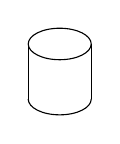
\begin{tikzpicture}%
    \draw (0.4, 0.7) ellipse (0.4 and 0.2);
    \draw (0.0, 0.0) arc (180:360:0.4 and 0.2);
    \draw (0.0, 0) -- (0.0, 0.7);
    \draw (0.8, 0) -- (0.8, 0.7);
\end{tikzpicture}}

% Public domain image https://commons.wikimedia.org/wiki/File:Symbol_thumbs_up.svg
\newcommand{\thumbsup}{\includegraphics[height=8pt]{images/thumbsup.pdf}}%

\hyphenation{time-stamp time-stamps}
